%%%%%%%%%%%%%%%%%%%%%%%%%%%%%%%%%%%%%%%%%%%%%%%%
%% Intro to LaTeX and Template for Homework Assignments
%% Quantitative Methods in Political Science
%% University of Mannheim
%% Fall 2019
%%%%%%%%%%%%%%%%%%%%%%%%%%%%%%%%%%%%%%%%%%%%%%%%

% created by Marcel Neunhoeffer & Sebastian Sternberg


% This template and tutorial will help you to write up your homework. It will also help you to use Latex for other assignments than this course's homework.

%%%%%%%%%%%%%%%%%%%%%%%%%%%%%%%%%%%%%%%%%%%%%%%%
% Before we get started
%%%%%%%%%%%%%%%%%%%%%%%%%%%%%%%%%%%%%%%%%%%%%%%%

% Make an account on overleaf.com and get started. No need to install anything.

%%%%%%%%%%%%%%%%%%%%%%%%%%%%%%%%%%%%%%%%%%%%%%%%
% Or if you want it the nerdy way...
% INSTALL LATEX: Before we can get started you need to install LaTeX on your computer.
				% Windows: http://miktex.org/download
				% Mac:         http://www.tug.org/mactex/mactex-download.html	
				% There a many more different LaTeX editors out there for both operating systems. I use TeXworks because it looks the same on Windows and Mac.
				

% SAVE THE FILE: The first thing you need to do is to save your LaTeX file in a directory as a .tex file. You will not be able to do anything else unless your file is saved. I suggest to save the .tex file in the same folder with your .R script and where you will save your plots from R to. Let's call this file template_homework1.tex and save it in your Week 1 folder.


% COMPILE THE FILE: After setting up your file, using your LaTeX editor (texmaker, texshop), you can compile your document using PDFLaTeX.
	% Compiling your file tells LaTeX to take the code you have written and create a pdf file
	% After compiling your file, in your directory will appear four new files, including a .pdf file. This is your output document.
	% It is good to compile your file regularly so that you can see how your code is translating into your document.
	
	
% ERRORS: If you get an error message, something is wrong in your code. Fix errors before they pile up!
	% As with error messages in R, google the exact error message if you have a question!
%%%%%%%%%%%%%%%%%%%%%%%%%%%%%%%%%%%%%%%%%%%%%%%%


% Now again for everyone...

% COMMANDS: 
	% To do anything in LaTeX, you must use commands
	% Commands tell LaTeX when to start your document, how you want your document to look, and how to format your document
	% Commands ALWAYS begin with a backslash \

% Everything following the % sign is a comment and will not be used by Latex to compile your document.
% This is very similar to # comments in R.

% Every .tex file usually consists of four parts.
% 1. Document Class
% 2. Packages
% 3. Header
% 4. Your Document

%%%%%%%%%%%%%%%%%%%%%%%%%%%%%%%%%%%%%%%%%%%%%%%%
% 1. Document Class
%%%%%%%%%%%%%%%%%%%%%%%%%%%%%%%%%%%%%%%%%%%%%%%%
 
 % The first command you will always have will declare your document class. This tells LaTeX what type of document you are creating (article, presentation, poster, etc). 
% \documentclass is the command
% in {} you specify the type of document
% in [] you define additional parameters
 
\documentclass[a4paper,12pt]{article} % This defines the style of your paper

% We usually use the article type. The additional parameters are the format of the paper you want to print it on and the standard font size. For us this is a4paper and 12pt.

%%%%%%%%%%%%%%%%%%%%%%%%%%%%%%%%%%%%%%%%%%%%%%%%
% 2. Packages
%%%%%%%%%%%%%%%%%%%%%%%%%%%%%%%%%%%%%%%%%%%%%%%%

% Packages are libraries of commands that LaTeX can call when compiling the document. With the specialized commands you can customize the formatting of your document.
% If the packages we call are not installed yet, TeXworks will ask you to install the necessary packages while compiling.

% First, we usually want to set the margins of our document. For this we use the package geometry. We call the package with the \usepackage command. The package goes in the {}, the parameters again go into the [].
\usepackage[top = 2.5cm, bottom = 2.5cm, left = 2.5cm, right = 2.5cm]{geometry} 

% Unfortunately, LaTeX has a hard time interpreting German Umlaute. The following two lines and packages should help. If it doesn't work for you please let me know.
\usepackage[T1]{fontenc}
\usepackage[utf8]{inputenc}

% The following two packages - multirow and booktabs - are needed to create nice looking tables.
\usepackage{multirow} % Multirow is for tables with multiple rows within one cell.
\usepackage{booktabs} % For even nicer tables.

% As we usually want to include some plots (.pdf files) we need a package for that.
\usepackage{graphicx} 

% The default setting of LaTeX is to indent new paragraphs. This is useful for articles. But not really nice for homework problem sets. The following command sets the indent to 0.
\usepackage{setspace}
\setlength{\parindent}{0in}

% Package to place figures where you want them.
\usepackage{float}

% The fancyhdr package let's us create nice headers.
\usepackage{fancyhdr}

\usepackage[utf8]{vietnam}

\usepackage{tikz}

\usepackage{graphicx}

\usepackage{listings}

\usepackage{amsmath}

\usepackage{hyperref}
\hypersetup{
    colorlinks=true,
    linkcolor=blue,
    filecolor=magenta,      
    urlcolor=cyan,
    pdftitle={Overleaf Example},
    pdfpagemode=FullScreen,
    }

\urlstyle{same}

\usepackage{xcolor}
\usepackage{tcolorbox}

% Import custom code block
\usepackage{graphicx}

% define listing code
\definecolor{codegreen}{rgb}{0,0.6,0}
\definecolor{codegray}{rgb}{0.5,0.5,0.5}
\definecolor{codepurple}{rgb}{0.58,0,0.82}
\definecolor{backcolour}{rgb}{0.95,0.95,0.92}

\lstdefinestyle{code}{
    backgroundcolor=\color{backcolour},   
    commentstyle=\color{codegreen},
    keywordstyle=\color{magenta},
    numberstyle=\tiny\color{codegray},
    stringstyle=\color{codepurple},
    basicstyle=\ttfamily\footnotesize,
    breakatwhitespace=false,         
    breaklines=true,                 
    captionpos=b,                    
    keepspaces=true,                 
    numbers=left,
    firstnumber=1,
    stepnumber=1,                    
    numbersep=5pt,                  
    showspaces=false,                
    showstringspaces=false,
    showtabs=false,                  
    tabsize=2,
    framesep=10pt,
    xleftmargin=10pt,
    xrightmargin=10pt,
    framexleftmargin=16pt,
    framextopmargin=2pt,
    framexbottommargin=2pt, 
    frame=tb, framerule=0pt,
}

\lstdefinestyle{algo}{
    backgroundcolor=\color{backcolour},   
    commentstyle=\color{codegreen},
    keywordstyle=\color{magenta},
    numberstyle=\tiny\color{codegray},
    stringstyle=\color{codepurple},
    basicstyle=\ttfamily\footnotesize\small\linespread{0.8},
    breakatwhitespace=false,         
    breaklines=true,                 
    captionpos=b,                    
    keepspaces=true,                 
    numbers=none,
    firstnumber=1,
    stepnumber=1,                    
    numbersep=5pt,                  
    showspaces=false,                
    showstringspaces=false,
    showtabs=false,                  
    tabsize=2,
    framesep=10pt,
    xleftmargin=10pt,
    xrightmargin=10pt,
    framexleftmargin=16pt,
    framextopmargin=2pt,
    framexbottommargin=2pt, 
    frame=tb, framerule=0pt,
    mathescape=true
}

\lstset{style=code}


%%%%%%%%%%%%%%%%%%%%%%%%%%%%%%%%%%%%%%%%%%%%%%%%
% 3. Header (and Footer)
%%%%%%%%%%%%%%%%%%%%%%%%%%%%%%%%%%%%%%%%%%%%%%%%

% To make our document nice we want a header and number the pages in the footer.

\pagestyle{fancy} % With this command we can customize the header style.

% \fancyhf{} % This makes sure we do not have other information in our header or footer.

% \lhead{\footnotesize QM 2019: Homework 1}% \lhead puts text in the top left corner. \footnotesize sets our font to a smaller size.

%\rhead works just like \lhead (you can also use \chead)
% \rhead{\footnotesize Lastname 1, Lastname 2 (\& Lastname 3)} %<---- Fill in your lastnames.

% Similar commands work for the footer (\lfoot, \cfoot and \rfoot).
% We want to put our page number in the center.
\cfoot{\footnotesize \thepage} 


%%%%%%%%%%%%%%%%%%%%%%%%%%%%%%%%%%%%%%%%%%%%%%%%
% 4. Your document
%%%%%%%%%%%%%%%%%%%%%%%%%%%%%%%%%%%%%%%%%%%%%%%%

% Now, you need to tell LaTeX where your document starts. We do this with the \begin{document} command.
% Like brackets every \begin{} command needs a corresponding \end{} command. We come back to this later.

\begin{document}


%%%%%%%%%%%%%%%%%%%%%%%%%%%%%%%%%%%%%%%%%%%%%%%%
%%%%%%%%%%%%%%%%%%%%%%%%%%%%%%%%%%%%%%%%%%%%%%%%

%%%%%%%%%%%%%%%%%%%%%%%%%%%%%%%%%%%%%%%%%%%%%%%%
% Title section of the document
%%%%%%%%%%%%%%%%%%%%%%%%%%%%%%%%%%%%%%%%%%%%%%%%

% For the title section we want to reproduce the title section of the Problem Set and add your names.

\thispagestyle{empty} % This command disables the header on the first page. 

\begin{tabular}{p{15.5cm}} % This is a simple tabular environment to align your text nicely 
{\large \bf Toán rời rạc và thuật toán} \\
Đại học Khoa học Tự nhiên \\
Khoa Toán - Cơ - Tin học \\ 
Khoa học dữ liệu K4 \\
Tháng 9 năm 2022  \\ 
\hline % \hline produces horizontal lines.
\\
\end{tabular} % Our tabular environment ends here.

\vspace*{0.3cm} % Now we want to add some vertical space in between the line and our title.

\begin{center} % Everything within the center environment is centered.
	{\Large \bf Bài tập số 1} % <---- Don't forget to put in the right number
	\vspace{2mm}
	
        % YOUR NAMES GO HERE
	{\bf Nguyễn Mạnh Linh, Nguyễn Thị Đông, Triệu Hồng Thúy} % <---- Fill in your names here!
		
\end{center}  

\vspace{0.4cm}

%%%%%%%%%%%%%%%%%%%%%%%%%%%%%%%%%%%%%%%%%%%%%%%%
%%%%%%%%%%%%%%%%%%%%%%%%%%%%%%%%%%%%%%%%%%%%%%%%

% Up until this point you only have to make minor changes for every week (Number of the homework). Your write up essentially starts here.

\section{Bài 1}


\section{Bài 2}

\subsection{Chia để trị}

\subsubsection{Ý tưởng}
Phương pháp chia để trị dựa trên 2 thao tác chính:
\begin{itemize}
    \item Chia (\textit{devide}): phân rã bài toán ban đầu thành các bài toán con có kích thước
    nhỏ hơn, có cùng cách giải.
    \item Trị (\textit{conque}): giải từng bài toán con (theo cách tương tự bài toán đầu - đệ
    qui) rồi tổng hợp các lời giải để nhận kết quả của bài toán ban đầu.
\end{itemize}

Việc “Phân rã”: thực hiện trên miền dữ liệu (chia miền dữ liệu thành các miền
nhỏ hơn tương đương 1 bài toán con)

\subsubsection{Mô hình và lược đồ}
Xét bài toàn $P$ trên miền dữ liệu $R$.

Gọi $D\_C(R)$ là thuật giải $P$ trên miền dữ liệu $R$.

Nếu $R$ có thể phân rã thành $n$ miền con: $R = R_1 \cup R_2 \cup ... \cup R_n$

Với $R_0$ là miền đủ nhỏ để  $D\_C(R)$ có lời giải, ta có lược đồ giải thuật chia để trị như sau:

\begin{lstlisting}[style=algo]
    Divide_Conque($R$):
        if($R = R_0$):
            solve Divide_Conque($R_0$)
        else
            divide $R$ to $R_1, R_2, ..., R_n$
            for ($i = 1, 2, ..., n$):
                Divide_Conque($R_i$)
            Combine and get result
    end
\end{lstlisting}

\subsubsection{Phân tích và đánh giá}
Để phân tích và đánh giá độ phức tạp của thuật toán, ta thực hiện 2 công đoạn

\begin{itemize}
    \item Xây dựng công thức truy hồi đánh giá độ phức tạp thuật toán
    \item Giải công thức truy hồi xác định độ phức tạp thuật toán.
        \begin{itemize}
            \item Phép thế liên tiếp
            \item Sử dụng định lí chính
        \end{itemize}
\end{itemize}


\subsubsection{Ví dụ}
Ta xét bài toán \textit{tìm kiếm nhị phân trên một mảng được sắp xếp}.

Cho dãy $n$ phần tử được sắp theo thứ tự (\textit{tăng dần}) và một giá trị $x$ 
bất kỳ. Kiểm tra xem phần tử  $x$ có trong dãy không?


\section{Bài 3}
Trong bài này chúng ta sẽ xem xét bài toán dóng hàng
toàn cục 2 chuỗi DNA sử dụng phương pháp quy hoạch động 
với giải thuật Needleman-Wunsch.

\subsection{Bài toán dòng hàng toàn cục}
Có nhiều cách để phát biểu bài toán dóng hàng trình tự 
(cho DNA, RNA hoặc 2 chuỗi kí tự). Hãy cùng điểm qua vài khái niệm.

\begin{itemize}
    \item Dóng hàng trình tự: là một cách sắp xếp trình tự của DNA,
    RNA hoặc protein để xác định các vùng giống nhau có thể là
    hệ quả của mối quan hệ chức năng, cấu trúc hoặc tiến hóa giữa
    các trình tự.
    \item Một cách dóng hàng của 2 chuỗi được thiết lập bằng cách thêm
    các khoảng trống (dấu cách) vào các vị trí bất kì trên 2 chuỗi này
    để chúng có cùng độ dài và không có 2 khoảng trống nào có cùng vị trí 
    trên 2 chuỗi
    \item Chuỗi con chung dài nhất (longest common subsequence, LCS):
    là chuỗi trình tự chứa nhiều kí tự giống nhau nhất của hai hay
    nhiều chuỗi.
\end{itemize}
Ví dụ một cách dóng hàng với 2 chuỗi S (\lstinline{interestingly}) 
và T (\lstinline{bioinformatics}) như sau
\begin{center}
    \lstinline{-i--nterestingly} \\
    \lstinline{bioinformatics--}
\end{center}

Một cách tổng quát, chúng ta có thể chấm điểm cho mỗi cặp kí tự được dóng hàng.
Gọi $\Sigma$ là tập các kí tự và "-" là kí tự đặc biệt kí hiệu cho dấu cách. 
Sự tương tự của các cặp kí tự trong 2 chuỗi có thể được biểu diễn thông qua 
một ma trận $\delta$ mà $\delta(x,y)$ là điểm của cặp $x$ và $y$ với 
$x, y \in \Sigma \cup \{-\}$. \\
Bài toán dóng hàng toàn cục có thể mô hình hóa bằng cách tìm một cách dóng hàng A
nào đó để cực đại $\sum_{\{x, y \} \in A} \delta(x,y)$. Cách dóng hàng này được
gọi là cách tối ưu (\textit{optimal alignment}). \\
Khi một cặp kí tự được sắp xếp và giống nhau, liên hệ giữa chúng
 được gọi là \textit{match}, ngược
lại gọi là \textit{mismatch}. Khi dấu cách được thêm vào chuỗi thứ nhất mối liên hệ 
là \textit{insert}, khi được thêm vào chuỗi thứ 2 thì được gọi là \textit{delete}. \\
Trong ví dụ trên chúng ta có 5 \textit{matches}, 6 \textit{mismatchs}, 3 \textit{inserts}
và 2 \textit{deletes}.

Chúng ta cùng xem xét một ví dụ về dóng hàng toàn cục. Xét ma trận điểm cho tập 
$\{-, A, C, G, T\}$ với $\delta(x, y) = 2, -1, -1, -1$ lần lượt cho match, mismatch, 
delete và insert. Xét 2 chuỗi DNA $S = ACAATCC$ và $T = AGCATGC$, một cách dóng hàng
khả dĩ như sau:
\begin{center}
    \lstinline{S = A-CAATCC} \\
    \lstinline{T = AGCA-TGC}
\end{center}
Cách dóng hàng trên có 5 matches, 1 mismatch, 1 insert và 1 delete. Vậy điểm tương tự của 
cách dòng hàng này là 7. Có thể kiểm tra được đây là điểm cực đại thế nên cách dóng hàng
này là một cách tối ưu. Cần chú ý là có thể có nhiều hơn một cách dóng hàng tối ưu. 
Ví dụ 1 cách khác cũng trả về điểm tương tự cực đại.
\begin{center}
    \lstinline{S = A-CAATCC} \\
    \lstinline{T = AGC-ATGC}
\end{center}

\begin{figure}[H] % places figure environment here   
    \centering % Centers Graphic
    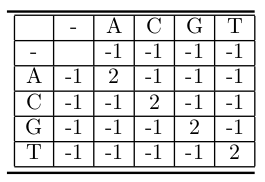
\includegraphics[width=0.3\textwidth]{./assets/score_matrix.png} 
    \caption{Ví dụ ma trận điểm tương tự} % Creates caption underneath graph
\end{figure}

\subsection{Giải thuật Needleman-Wunsch}
\subsubsection{Giải thuật}
Xét 2 chuỗi kí tự $S[1...n]$ và $T[1...m]$. Để tìm cách dóng hàng toàn cục tối ưu cho 
bài toán này chúng ta có thể nghĩ tới giải thuật vét cạn bằng cách sinh ra mọi cách 
dóng hàng và tìm xem cách nào có điểm cao nhất. Tuy nhiên cách tiếp cận này có thời
gian tính toán theo hàm mũ. Trong phần này, chúng ta sẽ xem xét một giải thuật hiệu quả
áp dụng \textit{quy hoạch đông} có tên là \textit{Needleman-Wunsch}. \\
Chúng ta thiết kế một hàm đệ quy (công thức truy hồi) $V(i,j)$ với 2 trường hợp: (1) $i = 0$ 
hoặc $j = 0$ và (2) cả $i > 0$ và $j > 0$. \\
Với trường hợp (1) khi $i = 0$ hoặc $j = 0$ chúng ta dóng hàng chuỗi bằng 1 chuỗi rỗng.
Hay nói cách khác là ta chỉ cần thêm hoặc xóa kí tự. Chúng ta có các phương trình:
\begin{equation}
    \begin{aligned}
        V(0, 0) &= 0 & \\
        V(0, j) &= V(0, j - 1) + \delta(-, T[j]) && \text{thêm j lần} \\
        V(i, 0) &= V(i -1, 0) + \delta(S[i], -) && \text{xóa i lần} 
    \end{aligned}
\end{equation}
Với trường hợp (2) khi cả $i > 0$ và $j > 0$, ta thấy rằng với một cách dóng hàng nào đó
của chuỗi $S[1...i]$ và $T[1...j]$ cặp kí tự cuối cùng phải thuộc 1 trong 3 loại 
match/mismatch (cả 2 đều là kí tự), insert hoặc delete. Để thu được điểm tối ưu ta chọn 
cách có điểm cực đại trong 3 trường hợp trên. Nghĩa là:
\begin{equation}
    V(i, j) = \max 
    \begin{cases}
        V(i - 1, j - 1) + \delta(S[i], T[j]) & \text{match/mismatch} \\
        V(i - 1, j) + \delta(S[i], -) & \text{delete} \\
        V(i, j - 1) + \delta(-, T[j]) & \text{insert} \\
    \end{cases}
\end{equation}
Điểm dóng hàng tối ưu của $[1...n]$ và $T[1...m]$ là $V(n,m)$. Điểm này có thể được tính bằng
cách điền đầy từng hàng vào bảng $V(1...n, 1...m)$ bằng các công thức truy hồi trên.

\begin{figure}[H] % places figure environment here   
    \centering % Centers Graphic
    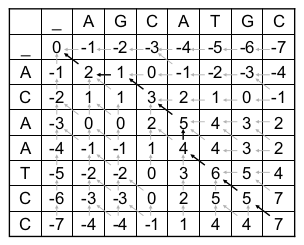
\includegraphics[width=0.4\textwidth]{./assets/dp.png} 
    \caption{Bảng điểm dóng hàng 2 chuỗi $S = ACAATCC$ và $T = AGCATGC$
    bằng giải thuật quy hoạch động Needleman-Wunsch} % Creates caption underneath graph
    \label{fig:dp_track}
\end{figure}

Hình trên là bảng $V$ cho 2 chuỗi $S = ACAATCC$ và $T = AGCATGC$.
Chúng ta có thể tính lần lượt giá trị của các ô trong bảng, ví dụ $V(1, 1)$ là giá trị 
lớn nhất trong tập $\{0+2, -1-1, -1-1\}$. Sau khi điền đầy các ô ta có $V(7,7) = 7$ là 
giá trị của ô dưới cùng bên phải hay chính là điểm của cách dóng hàng tối ưu.

Để tìm ngược lại cách dóng hàng tối ưu, với mỗi ô trong bảng ta vẽ các mũi tên để biểu 
diễn sự tương quan giữa các cặp. Ta vẽ mũi tên chéo, ngang và dọc lần lượt cho các trường
hợp match, insert và delete. Ví dụ giá trị tại $V(1,1)$ thu được bởi $V(0,0) + 2$, chúng 
ta vẽ 1 mũi tên chéo. Với ô $V(3,2)$, có 2 cách có giá trị điểm bằng điểm lớn nhất nên 
ta vẽ cả 2 mũi tên chéo và dọc. Để thu được cách dóng hàng tối ưu ta cần quay lui từ ô 
$V(7,7)$ về ô $V(0,0)$. Nếu mũi tên là chéo, 2 kí tự được dóng hàng. Với mũi tên ngang và
dọc thì lần lượt là delete và insert. Ta thu được đường quay lui là đường mũi tên in đậm 
trong hình \ref{fig:dp_track} theo đường $7 \to 5 \to 6 \to 4 \to 5 \to 3 \to 1 \to 0$.
Tương ứng ta thu được cách dóng hàng tối ưu:

\begin{center}
    \lstinline{A-CAATCC} \\
    \lstinline{AGCA-TGC}
\end{center}

\subsubsection{Thời gian tính toán}
Như đã trình bày trong phần trước, thuật toán Needleman-Wunsch có thời gian tính toán là $O(nm)$
khi giải bài toán dóng hàng toàn cục do chúng ta cần điền vào toàn bộ các ô trong bảng điểm 
dòng hàng có kích thước $n \times m$

\subsection{Triển khai thuật toán}
Trong phần này chúng ta sẽ đưa ra mã giả cài đặt thuật toán Needleman-Wunsch để lập bảng điểm
dóng hàng và trình bày cách quay lui để đưa ra kết quả dóng hàng 2 chuỗi DNA. \\
Thay vì gọi là \textit{bảng} như phần trước, chung ta sẽ xây dựng một 
\textit{ma trận} $V$ gọi là ma trận \textit{score}.
Ở đây ta kí hiệu $v[i, j]$ là thành phần $v_{i,j}$ của ma trận $V$,
$s[i]$ là kí tự tại chỉ số $i$ của chuỗi $s$ (lưu ý chỉ số đánh từ $0$). \\
Trước hết là mã giả để  xây dựng ma trận $V$ hay nói cách khác là điền đầy 
bảng điểm dóng hàng của 2 chuỗi $s$ và $t$. \\

\begin{lstlisting}[style=algo]
    // alias for backtracking arrows
    left, up, dia = 1, 2, 3 

    // define score for characters status
    match, mismatch, insert, delete = 2, -1, -1, -1

    delta(a, b):
        // define score
        if a == b:
            return match
        if '-' == a:
            return insert
        if '-' == b:
            return delete
        return mismatch
    end

    node_score(s, t, node, i, j):
        // calculate score of node[i, j]
        score_match_mismatch = node[i-1, j-1] \
            + delta(s[i], t[j])
        score_delete = node[i-1, j] + delta(s[i], '-')
        score_insert = node[i, j-1] + delta(s[i], '-')
        return max([score_match_mismatch, 
                    score_delete, 
                    score_insert])
    end


    lsc(s, t):
        // fill the score table
        n = length of s
        m = length of t
        backtrack = zero matrix with size $(n+1) \times (m+1)$
        v = zero matrix with size $(n+1) \times (m+1)$
        s = '-' + s
        t = '-' + t

        for i from 0 to n:
            v[i, 0] = -i

        for j from 0 to m:
            v[0, j] = -j

        for i from 1 to n:
            for j from 0 to m:
                v[i, j] = node_score(s, t, v, i, j)
                if v[i, j] == v[i-1, j] + delta(s[i], '-'):
                    backtrack[i, j] = up
                elif v[i, j] == v[i, j-1] + delta('-', t[j]):
                    backtrack[i, j] = left
                else:
                    backtrack[i, j] = dia

        return v, backtrack
    end
\end{lstlisting}

Tiếp theo ta có mã giả cho quá trình quay lui để đưa ra kết quả dòng hàng
\begin{lstlisting}[style=algo]
    output(s, t, backtrack):
        // return 2 aligned sequences
        n = length of s
        m = length of t
        source, target = s, t
        i, j = n, m
        while i > 0 and j > 0:
            if backtrack[i, j] == left:
                inserting '-' to source at index $(j-1)$
                j = j - 1
                continue
            if backtrack[i, j] == up:
                inserting '-' to target at index $(i-1)$
                i = i - 1
                continue
            i = i - 1
            j = j - 1
        return source, target
    end
\end{lstlisting}

Cuối cùng là \href{https://github.com/batman0911/dma_homework/blob/master/hw_01/src/sequence.ipynb}{python code} 
cài đặt thuật toán.  





% % Now we also want to include the graph in our write up.
%  \begin{figure}[H] % places figure environment here   
%     \centering % Centers Graphic
%     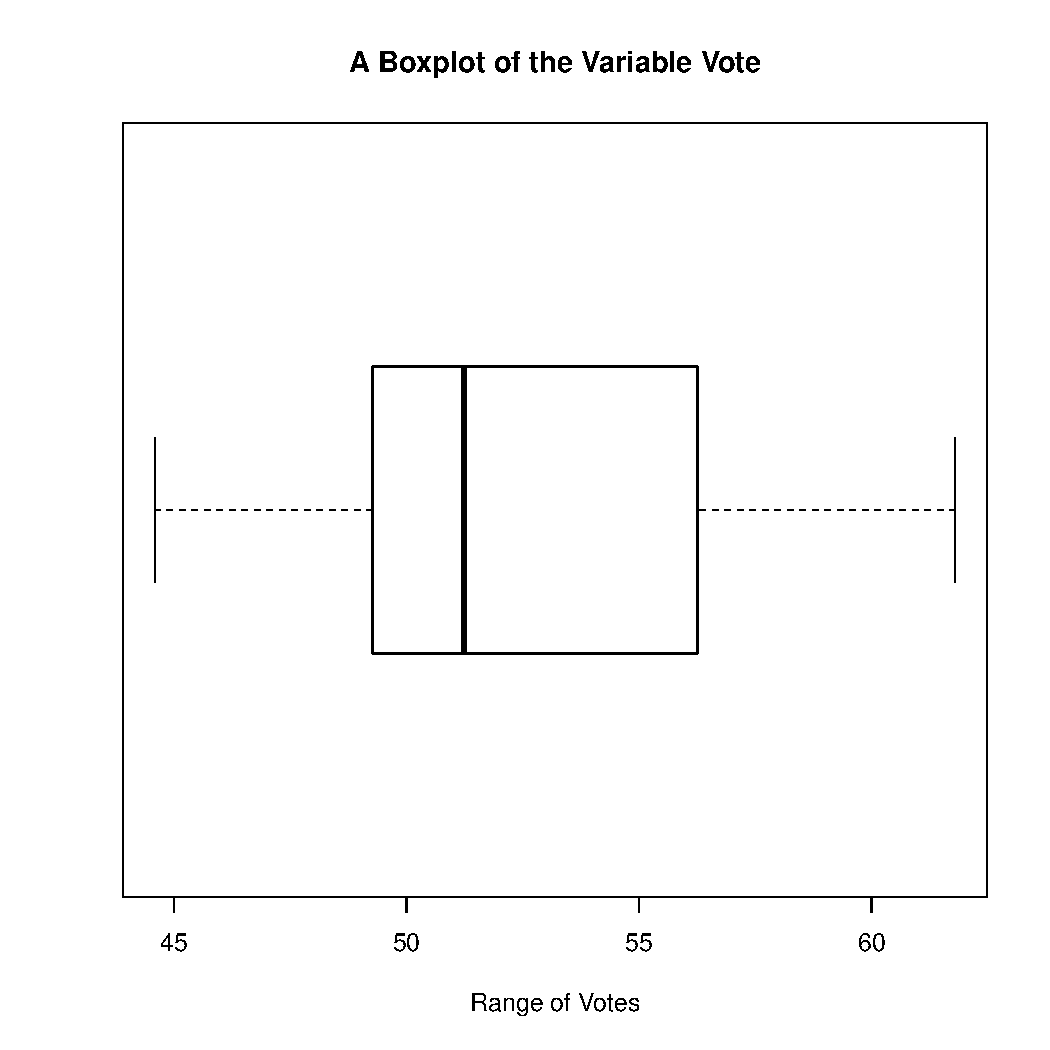
\includegraphics[width=0.9\textwidth]{box1.pdf} 
%     \caption{Boxplot of Incumbent Vote share} % Creates caption underneath graph
%   \end{figure}


% % Now all we need to answer the question is a neat table. The easiest way to get a nice looking table is to browse to http://www.tablesgenerator.com. Generate your table just like in Word or any other WYSIWYG editor. Then copy and include the code here. I already did that for you.

% \begin{table}[H]
% \centering
% \begin{tabular}{llllllll}
% \multicolumn{1}{c}{\textbf{Variable}} & \multicolumn{1}{c}{\textit{Mean}} & \multicolumn{1}{c}{\textit{Median}} & \textit{Mode} & \textit{Var} & \textit{SD} & \textit{Range} & \textit{IQR} \\ \hline
% Vote                                  & x                                 & x                                   & x             & x            & x           & x              & x            \\
% Growth                                & x                                 & x                                   & x             & x            & x           & x              & x           
% \end{tabular}
% \caption{Measures of central tendency and variability.}
% \label{my-label}
% \end{table}
% You just have to exchange the x for the right value.

\end{document}
